% Options for packages loaded elsewhere
\PassOptionsToPackage{unicode}{hyperref}
\PassOptionsToPackage{hyphens}{url}
%
\documentclass[
]{article}
\usepackage{lmodern}
\usepackage{amssymb,amsmath}
\usepackage{ifxetex,ifluatex}
\ifnum 0\ifxetex 1\fi\ifluatex 1\fi=0 % if pdftex
  \usepackage[T1]{fontenc}
  \usepackage[utf8]{inputenc}
  \usepackage{textcomp} % provide euro and other symbols
\else % if luatex or xetex
  \usepackage{unicode-math}
  \defaultfontfeatures{Scale=MatchLowercase}
  \defaultfontfeatures[\rmfamily]{Ligatures=TeX,Scale=1}
\fi
% Use upquote if available, for straight quotes in verbatim environments
\IfFileExists{upquote.sty}{\usepackage{upquote}}{}
\IfFileExists{microtype.sty}{% use microtype if available
  \usepackage[]{microtype}
  \UseMicrotypeSet[protrusion]{basicmath} % disable protrusion for tt fonts
}{}
\makeatletter
\@ifundefined{KOMAClassName}{% if non-KOMA class
  \IfFileExists{parskip.sty}{%
    \usepackage{parskip}
  }{% else
    \setlength{\parindent}{0pt}
    \setlength{\parskip}{6pt plus 2pt minus 1pt}}
}{% if KOMA class
  \KOMAoptions{parskip=half}}
\makeatother
\usepackage{xcolor}
\IfFileExists{xurl.sty}{\usepackage{xurl}}{} % add URL line breaks if available
\IfFileExists{bookmark.sty}{\usepackage{bookmark}}{\usepackage{hyperref}}
\hypersetup{
  pdftitle={Estatística e Análise de Dandos},
  pdfauthor={Lirielly Nascimento e Pedro Magalhães},
  hidelinks,
  pdfcreator={LaTeX via pandoc}}
\urlstyle{same} % disable monospaced font for URLs
\usepackage[margin=2.5cm]{geometry}
\usepackage{longtable,booktabs}
% Correct order of tables after \paragraph or \subparagraph
\usepackage{etoolbox}
\makeatletter
\patchcmd\longtable{\par}{\if@noskipsec\mbox{}\fi\par}{}{}
\makeatother
% Allow footnotes in longtable head/foot
\IfFileExists{footnotehyper.sty}{\usepackage{footnotehyper}}{\usepackage{footnote}}
\makesavenoteenv{longtable}
\usepackage{graphicx}
\makeatletter
\def\maxwidth{\ifdim\Gin@nat@width>\linewidth\linewidth\else\Gin@nat@width\fi}
\def\maxheight{\ifdim\Gin@nat@height>\textheight\textheight\else\Gin@nat@height\fi}
\makeatother
% Scale images if necessary, so that they will not overflow the page
% margins by default, and it is still possible to overwrite the defaults
% using explicit options in \includegraphics[width, height, ...]{}
\setkeys{Gin}{width=\maxwidth,height=\maxheight,keepaspectratio}
% Set default figure placement to htbp
\makeatletter
\def\fps@figure{htbp}
\makeatother
\setlength{\emergencystretch}{3em} % prevent overfull lines
\providecommand{\tightlist}{%
  \setlength{\itemsep}{0pt}\setlength{\parskip}{0pt}}
\setcounter{secnumdepth}{5}
%----------------------------------------------------------------------------------------
%	REQUIRED PACKAGES
%
% pdfpages:(http://mirrors.up.pt/pub/CTAN/macros/latex/contrib/pdfpages/pdfpages.pdf)
% geometry: (https://www.overleaf.com/learn/latex/Page_size_and_margins)
% fancyhdr: (https://www.overleaf.com/learn/latex/Headers_and_footers)
% xcolor: (https://www.overleaf.com/learn/latex/Using_colours_in_LaTeX)
% titlesec: https://www.overleaf.com/learn/latex/Sections_and_chapters
%----------------------------------------------------------------------------------------

\usepackage{pdfpages} %allows the introduction of pdf pages 
\usepackage{fancyhdr} %changes headers and footers
\usepackage{xcolor} %Lets set different colors for the document
\usepackage{titlesec} %customizes chapters(book) and sections(article)
\usepackage{tikz}
\usepackage{fontspec} %customizes fonts
\usepackage{graphicx} %add graphical elements
\usepackage{background} %customizes documents backgrounds
\usepackage{lastpage}
\usepackage{caption} % allows image caption costumization
\usepackage{blindtext}
\usepackage[most]{tcolorbox}
\tcbuselibrary{skins}
\usepackage{multicol} % allows more than one column on text
\usepackage{enumitem} % Allows to change lists %>% 
\usepackage[default]{opensans}
\usepackage{setspace}\setstretch{1.25}
\usepackage{float}
\floatplacement{figure}{H}
%\usepackage{setspace}\singlespacing

%----------------------------------------------------------------------------------------
%	FONTS FORMAT
%----------------------------------------------------------------------------------------

\setmainfont[SizeFeatures={Size=10}]{Open Sans}

%----------------------------------------------------------------------------------------
%	DOCUMENT COLORS
%----------------------------------------------------------------------------------------

\definecolor{DarkPurple}{HTML}{680c62}
\definecolor{MediumPurple}{HTML}{a8139d}
\definecolor{LightPurple}{HTML}{c26cf0}
\definecolor{Grey}{HTML}{bfbfbf}
\definecolor{lightGreen}{HTML}{ddeedd}
\definecolor{mediumGreen}{HTML}{77bb77}

\definecolor{DarkGray}{HTML}{403D3C}
\definecolor{AtomicGreen}{HTML}{10FF10}

%----------------------------------------------------------------------------------------
%	SECTION FORMAT
%----------------------------------------------------------------------------------------

\titleformat{\section}[block]
  {\titlerule\addvspace{4pt}\normalfont\fontsize{12}{12}\bfseries}
  {\thesection\enspace}{0pt}{}[\vspace{2pt}\titlerule]

\titleformat*{\section}{\color{DarkGray}\fontsize{16}{16}\normalfont\bfseries}
\titleformat*{\subsection}{\color{DarkGray}\fontsize{12}{12}\normalfont\bfseries}
\titleformat*{\subsubsection}{\color{AtomicGreen}\fontsize{10}{10}\normalfont\bfseries}

\titlespacing*{\section}{0pt}{30pt}{50pt}
\titlespacing*{\subsection}{0pt}{40pt}{10pt}

%----------------------------------------------------------------------------------------
%	CUSTOM HEADER AND FOOTER
%----------------------------------------------------------------------------------------

\pagestyle{fancy}
\fancyhf{} %clear all headers and footer fields
%\fancyhead[RO,RE]{\textcolor{DarkGray}{math.marketing}}
\fancyhead[LO,LE]{\textcolor{DarkGray}{\thepage}}
\renewcommand{\headrulewidth}{0pt} %Eliminates header row that is part of the default


\backgroundsetup{
  scale=1.3,
  opacity=1,
  angle=0,
  position=current page.south,
  hshift=0pt, %-27
  vshift=20pt,
  contents={%
  \small\sffamily%
  \begin{minipage}{1\textwidth}
  \includegraphics[scale=0.5]{theme/images/footer.png}
  \end{minipage}%
  }
}

%----------------------------------------------------------------------------------------
%	CUSTOM IMAGE FORMATING
%----------------------------------------------------------------------------------------

\captionsetup[figure]{name=Fig.}

%----------------------------------------------------------------------------------------
%	COVER PAGE
%----------------------------------------------------------------------------------------

\AtBeginDocument{\let\maketitle\relax}

%----------------------------------------------------------------------------------------
%	NEW COMMANDS
%-------------------------------------------------------------------------------------

% http://texdoc.net/texmf-dist/doc/latex/tcolorbox/tcolorbox.pdf

\newcommand{\impactBox}[2]{
  \begin{tcolorbox}[width=\textwidth,
  fonttitle = \sffamily\bfseries\large, 
  colframe={mediumGreen},
  colback={lightGreen},
  title={#1},
  sharp corners]  
  \textsc{#2}
  \end{tcolorbox} 
}

\newcommand{\attentionBox}[1]{
  \begin{tcolorbox}[fonttitle = \sffamily\bfseries\large,
  bicolor,
  sidebyside,
  lefthand width=0.5cm,
  sharp corners,
  boxrule=.4pt,
  colback=yellow!30,
  colbacklower=yellow!20]
    \includegraphics[scale=5]{theme/images/attention-sign.png}
  \tcblower
    \textsc{#1}%
  \end{tcolorbox}
}
\usepackage[]{natbib}
\bibliographystyle{plainnat}

\title{Estatística e Análise de Dandos}
\usepackage{etoolbox}
\makeatletter
\providecommand{\subtitle}[1]{% add subtitle to \maketitle
  \apptocmd{\@title}{\par {\large #1 \par}}{}{}
}
\makeatother
\subtitle{Trabalho Prático}
\author{Lirielly Nascimento e Pedro Magalhães}
\date{18/04/2022}

\begin{document}
\NoBgThispage %does not apply background

\includepdf{theme/images/cover.pdf}
\maketitle



{
\setcounter{tocdepth}{3}
\tableofcontents
}
\hypertarget{introduuxe7uxe3o}{%
\section{Introdução}\label{introduuxe7uxe3o}}

\hypertarget{descriuxe7uxe3o-dos-dados}{%
\subsection{Descrição dos Dados}\label{descriuxe7uxe3o-dos-dados}}

O Complexo Bushveld, a maior intrusão máfico-ultramáfica em camadas do mundo, é anfitrião de numerosas camadas de cromitita, lateralmente contínuas e quimicamente semelhantes. Com base em sua posição estratigráfica as camadas são subdivididas em um grupo inferior, médio e superior (LG, MG e UG). Dentro desses grupos as camadas são numeradas sucessivamente -- da base ao topo de cada grupo.

Tentativas de discriminar entre camadas únicas com base em sua composição falharam - principalmente devido à sobreposição significativa de campos de composição, por exemplo, de agrupamentos minerais de cromitita e química mineral de cromita entre camadas (vizinhas).

O conjunto de dados que utilizaremos foi fornecido pela Cronimet SA (Pty) Ltd., compreendendo em um grande banco de dados geoquímico (N = 1205) de cromitita de interseções de núcleo de perfuração e abrange 14 camadas de cromitita distintas (LG-1 -- LG-7, MG-1 -- MG-4, incluindo o LG-6A, MG-4A, MG-4Z) da Mina Thaba (que pode ser identificada na imagem abaixo), uma mina de cromita localizada no limbo ocidental do Complexo Bushveld. Os dados mostrados são restritos a cromitita maciça, excluindo paredões ou camadas suspensas de paredes, mas as análises podem conter intercalações de silicato finos (até alguns cm de espessura), separações de piroxenita, oikocristais de piroxênio, etc. Estes permanecem no conjunto de dados em ordem para representar toda a gama de possíveis composições de cromitita dentro da mina.

Durante a exploração na Mina Thaba, a composição das camadas de cromitita é rotineiramente restrita por apenas seis óxidos de elementos principais (Cr2O3, FeO, Al2O3, MgO, SiO2, CaO) e P. Além disso, o banco de dados da empresa contém valores para concentrações de Au e PGE, incluindo Pt, Pd, Rh, Ru e Ir. O banco de dados foi previamente filtrado para quaisquer valores ausentes (como ``não analisado'' ou ``abaixo do limite de detecção'') entre os principais óxidos do elemento e o PGE.

\begin{figure}
\centering
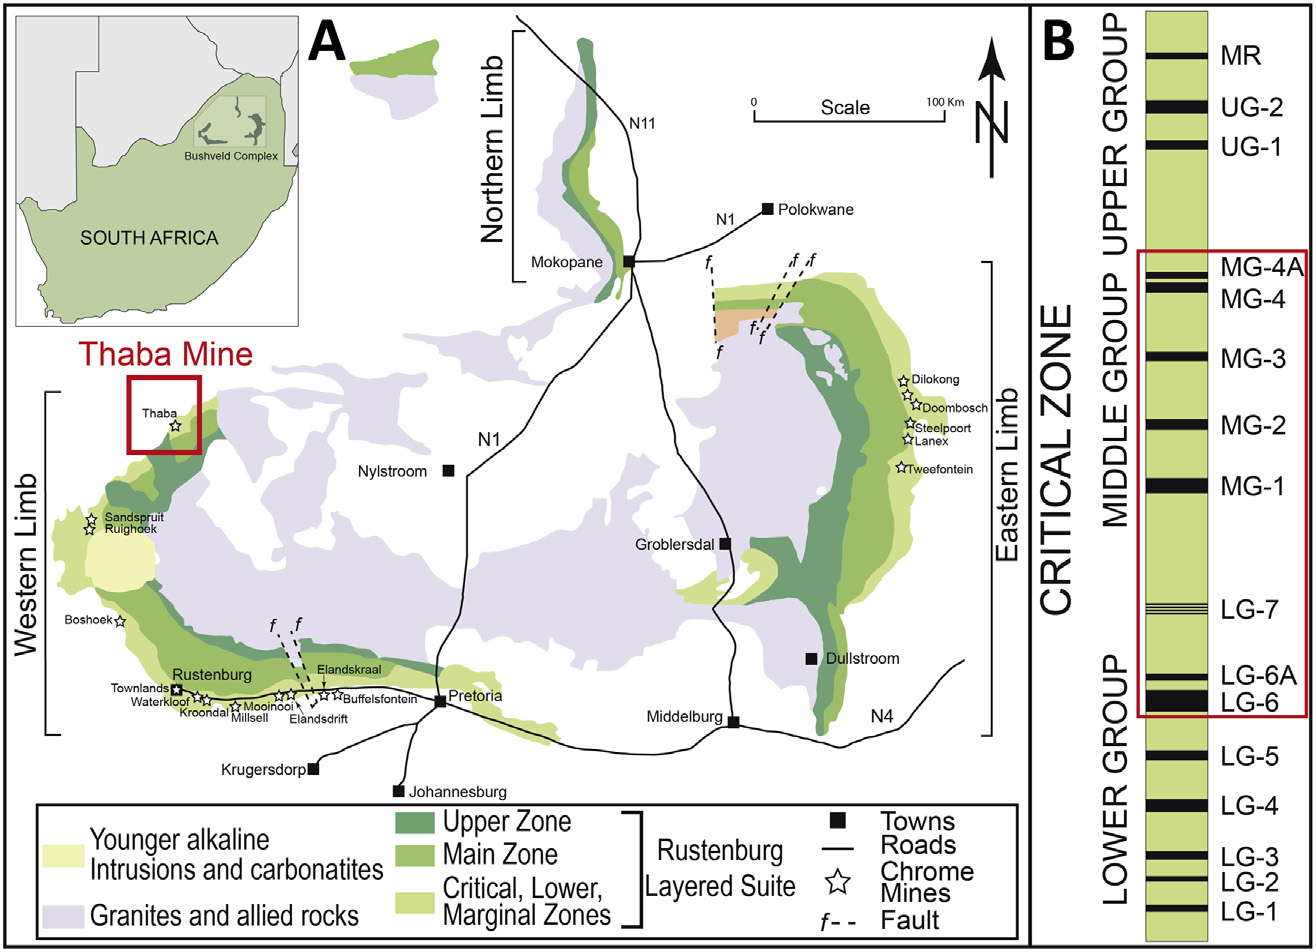
\includegraphics{./data/CB.png}
\caption{Imagem 1: Complexo Bushveld}
\end{figure}

Neste trabalho realizaremos algumas análises, dentre elas: análise de correlação, análise de componentes principais e análise do qui-quadrado. O nosso intuito com essas análises é verificar se conseguimos reduzir a dimensionalidade dos dados (variáveis numéricas) e obter um novo espaço de representação com uma boa representatividade das variáveis originais com as componentes criadas. Mais ainda, que as componentes selecionadas, as que explicam parte importante da dispersão, consigam mostrar a influência dos componentes geoquímicos nas amostras de cromitita.

O dataset contendo os dados analisados neste trabalho pode ser acessado no seguinte \href{https://www.kaggle.com/saurabhshahane/multivariate-geochemical-classification}{link}.

\hypertarget{definiuxe7uxe3o-das-variuxe1veis}{%
\subsection{Definição das variáveis}\label{definiuxe7uxe3o-das-variuxe1veis}}

\begin{longtable}[]{@{}
  >{\raggedright\arraybackslash}p{(\columnwidth - 4\tabcolsep) * \real{0.1633}}
  >{\raggedright\arraybackslash}p{(\columnwidth - 4\tabcolsep) * \real{0.7551}}
  >{\raggedright\arraybackslash}p{(\columnwidth - 4\tabcolsep) * \real{0.0816}}@{}}
\toprule
\begin{minipage}[b]{\linewidth}\raggedright
Variável
\end{minipage} & \begin{minipage}[b]{\linewidth}\raggedright
Descrição
\end{minipage} & \begin{minipage}[b]{\linewidth}\raggedright
Tipo da variável
\end{minipage} \\
\midrule
\endhead
HoleType & Tipo do furo que foi coletada a amostra & Categórica \\
MaxDepth & Profundidade máxima da coleta da amostra & Categórica \\
DepthFrom & Profundidade inicial da coleta da amostra & Numérica \\
DepthTo & Profundidade final da coleta da amostra & Numérica \\
Cr2O3\_\% & Percentual de Óxido de Cromo presente na amostra & Numérica \\
FeO\_\% & Percentual de Óxido de Ferro presente na amostra & Numérica \\
SiO2\_\% & Percentual de Dióxido de Silício presente na amostra & Numérica \\
MgO\_\% & Percentual de Óxido de Magnésio presente na amostra & Numérica \\
Al2O3\_\% & Percentual de Óxido de Alumínio presente na amostra & Numérica \\
CaO\_\% & Percentual de Óxido de Cálcio presente na amostra & Numérica \\
P\_\% & Percentual de Fósforo presente na amostra & Numérica \\
Au\_ICP\_ppm & Partes por milhão de ICP (Plasma Acoplado Indutivamente) de Ouro & Numérica \\
Pt\_ICP\_ppm & Partes por milhão de ICP (Plasma Acoplado Indutivamente) de Platina & Numérica \\
Pd\_ICP\_ppm & Partes por milhão de ICP (Plasma Acoplado Indutivamente) de Paládio & Numérica \\
Rh\_ICP\_ppm & Partes por milhão de ICP (Plasma Acoplado Indutivamente) de Ródio & Numérica \\
Ir\_ICP\_ppm & Partes por milhão de ICP (Plasma Acoplado Indutivamente) de Irídio & Numérica \\
Ru\_ICP\_ppm & Partes por milhão de ICP (Plasma Acoplado Indutivamente) de Ruténio & Numérica \\
Stratigraphy & Posição estratigráfica das camadas de cromitita dentro da Zona Crítica a partir da base para cima & Categórica \\
\bottomrule
\end{longtable}

\newpage

\newpage

\hypertarget{data-exploration}{%
\section{Data Exploration}\label{data-exploration}}

\hypertarget{holetype}{%
\subsection{HoleType}\label{holetype}}

\begin{center}\includegraphics{_main_files/figure-latex/unnamed-chunk-4-1} \end{center}

A variável \textbf{Holetype} que representa o tipo do buraco feito para coleta da amostra de cromitita em uma das sessõe da mina do complexo de Bushveld. A variável é categórica sendo que a maior prediminância da classe sendo o buraco feito por meio de um \textbf{poço artesiano} e a outra classe sendo o buraco feito por meio de \textbf{deflexão}.

\hypertarget{maxdepth}{%
\subsection{MaxDepth}\label{maxdepth}}

\textbf{MaxDepth} é a profundidade máxima do buraco utilizado para coleta da amostra de cromitita para a análise química. A váriável é categórica sendo que as classes \textbf{``Low''} e \textbf{``Middle''} tem praticamente a mesma proporção e a classe \textbf{``Depth''} tem aproximadamente o dobro da proporção das outras duas.

\hypertarget{depthfrom}{%
\subsection{DepthFrom}\label{depthfrom}}

\begin{center}\includegraphics{_main_files/figure-latex/unnamed-chunk-6-1} \end{center}

\textbf{DepthFrom} é a profundidade inicial de onde a amostra de cromitita foi coletada para a análise química. A váriável é contínua com distribuição gamma. O box-plot indica a presença de outliers, mas no contexto da coleta de amostras de cromitita para análise quimica esses valores não se confirmam como outliers e sim como prováveis de acontecer. Observamos por meio da distribuição desta variável que temos alguns valores com grande magnitude e desta forma a mediana e os valores máximo e mínimo são boas medidas de tendência central.

\hypertarget{depthto}{%
\subsection{DepthTo}\label{depthto}}

\begin{center}\includegraphics{_main_files/figure-latex/unnamed-chunk-7-1} \end{center}

\textbf{DepthTo} é a profundidade final de onde a amostra de cromitita foi coletada para a análise química. A váriável é contínua com distribuição gamma. O box-plot indica a presença de outliers, mas no contexto da coleta de amostras de cromitita para análise quimica esses valores não se confirmam como outliers e sim como prováveis de acontecer. Observamos por meio da distribuição desta variável que temos alguns valores com grande magnitude e desta forma a mediana e os valores máximo e mínimo são boas medidas de tendência central.

\hypertarget{cr2o3_}\label{cr2o3_}}

\begin{center}\includegraphics{_main_files/figure-latex/unnamed-chunk-8-1} \end{center}

\textbf{Cr2O3\_\%} representa o percentual de \textbf{óxido de cromo} contido na amostra de cromitita analisada. A váriável é contínua com distribuição bimodal, o box-plot sugere a presença de outliers. Por possuir alguns valores de grande amplitude a mediana e os valores máximo e mínimo são boas medidas de tendência central.

\hypertarget{feo_}\label{feo_}}

\begin{center}\includegraphics{_main_files/figure-latex/unnamed-chunk-9-1} \end{center}

\textbf{FeO\_\%} representa o percentual de \textbf{óxido de ferro} contido na amostra de cromitita analisada. A váriável é contínua com distribuição normal, o box-plot sugere a presença de outliers. Como a distribuição desta variável se assemelha a uma distribuição normal a média e o desvio padrão são boas medidas de tendência central.

\hypertarget{sio2_}\label{sio2_}}

\begin{center}\includegraphics{_main_files/figure-latex/unnamed-chunk-10-1} \end{center}

\textbf{SiO2\_\%} representa o percentual de \textbf{dióxido de silício} contido na amostra de cromitita analisada. A váriável é contínua com distribuição bimodal, o box-plot sugere a presença de outliers. E, por possuir alguns valores de grande amplitude a mediana e os valores máximo e mínimo são boas medidas de tendência central.

\hypertarget{mgo_}\label{mgo_}}

\begin{center}\includegraphics{_main_files/figure-latex/unnamed-chunk-11-1} \end{center}

\textbf{MgO\_\%} representa o percentual de \textbf{óxido de magnésio} contido na amostra de cromitita analisada. A váriável é contínua com distribuição normal, o box-plot sugere a presença de outliers. Como a distribuição desta variável se assemelha a uma distribuição normal a média e o desvio padrão são boas medidas de tendência central.

\hypertarget{al2o3_}\label{al2o3_}}

\begin{center}\includegraphics{_main_files/figure-latex/unnamed-chunk-12-1} \end{center}

\textbf{Al2O3\_\%} representa o percentual de \textbf{óxido de alumínio} contido na amostra de cromitita analisada. A váriável é contínua com distribuição bimodal, o box-plot sugere a presença de outliers. E, por possuir alguns valores de grande amplitude a mediana e os valores máximo e mínimo são boas medidas de tendência central.

\hypertarget{cao_}\label{cao_}}

\begin{center}\includegraphics{_main_files/figure-latex/unnamed-chunk-13-1} \end{center}

\textbf{CaO\_\%} representa o percentual de \textbf{óxido de cálcio} contido na amostra de cromitita analisada. A váriável é contínua com distribuição bimodal, o box-plot sugere a presença de outliers. E, por possuir alguns valores de grande amplitude a mediana e os valores máximo e mínimo são boas medidas de tendência central.

\hypertarget{p_}\label{p_}}

\begin{center}\includegraphics{_main_files/figure-latex/unnamed-chunk-14-1} \end{center}

\textbf{P\_\%} representa o percentual de \textbf{fósfoto} contido na amostra de cromitita analisada. A váriável é contínua com distribuição similar a uma gamma ou poisson, o box-plot sugere a presença de outliers. E, por possuir alguns valores de grande amplitude a mediana e os valores máximo e mínimo são boas medidas de tendência central.

\hypertarget{au_icp_ppm}{%
\subsection{Au\_ICP\_ppm}\label{au_icp_ppm}}

\begin{center}\includegraphics{_main_files/figure-latex/unnamed-chunk-15-1} \end{center}

\textbf{Au\_ICP\_ppm} representa as partes por milhão de ICP (Plasma Acoplado Indutivamente) de \textbf{ouro} contido na amostra de cromitita analisada. A váriável é contínua com distribuição similar a uma gamma ou poisson, o box-plot sugere a presença de outliers. E, por possuir alguns valores de grande amplitude a mediana e os valores máximo e mínimo são boas medidas de tendência central.

\hypertarget{pt_icp_ppm}{%
\subsection{Pt\_ICP\_ppm}\label{pt_icp_ppm}}

\begin{center}\includegraphics{_main_files/figure-latex/unnamed-chunk-16-1} \end{center}

\textbf{Pt\_ICP\_ppm} representa as partes por milhão de ICP (Plasma Acoplado Indutivamente) de \textbf{platina} contido na amostra de cromitita analisada. A váriável é contínua com distribuição bimodal, o box-plot sugere a presença de outliers. E, por possuir alguns valores de grande amplitude a mediana e os valores máximo e mínimo são boas medidas de tendência central.

\hypertarget{pd_icp_ppm}{%
\subsection{Pd\_ICP\_ppm}\label{pd_icp_ppm}}

\begin{center}\includegraphics{_main_files/figure-latex/unnamed-chunk-17-1} \end{center}

\textbf{Pd\_ICP\_ppm} representa as partes por milhão de ICP (Plasma Acoplado Indutivamente) de \textbf{paládio} contido na amostra de cromitita analisada. A váriável é contínua com distribuição gamma, o box-plot sugere a presença de outliers. E, por possuir alguns valores de grande amplitude a mediana e os valores máximo e mínimo são boas medidas de tendência central.

\hypertarget{rh_icp_ppm}{%
\subsection{Rh\_ICP\_ppm}\label{rh_icp_ppm}}

\begin{center}\includegraphics{_main_files/figure-latex/unnamed-chunk-18-1} \end{center}

\textbf{Rh\_ICP\_ppm} representa as partes por milhão de ICP (Plasma Acoplado Indutivamente) de \textbf{ródio} contido na amostra de cromitita analisada. A váriável é contínua com distribuição gamma, o box-plot sugere a presença de outliers. E, por possuir alguns valores de grande amplitude a mediana e os valores máximo e mínimo são boas medidas de tendência central.

\hypertarget{ir_icp_ppm}{%
\subsection{Ir\_ICP\_ppm}\label{ir_icp_ppm}}

\begin{center}\includegraphics{_main_files/figure-latex/unnamed-chunk-19-1} \end{center}

\textbf{Ir\_ICP\_ppm} representa as partes por milhão de ICP (Plasma Acoplado Indutivamente) de \textbf{irídio} contido na amostra de cromitita analisada. A váriável é contínua com distribuição bimodal, o box-plot sugere a presença de outliers. E, por possuir alguns valores de grande amplitude a mediana e os valores máximo e mínimo são boas medidas de tendência central.

\hypertarget{ru_icp_ppm}{%
\subsection{Ru\_ICP\_ppm}\label{ru_icp_ppm}}

\begin{center}\includegraphics{_main_files/figure-latex/unnamed-chunk-20-1} \end{center}

\textbf{Ru\_ICP\_ppm} representa as partes por milhão de ICP (Plasma Acoplado Indutivamente) de \textbf{ruténio} contido na amostra de cromitita analisada. A váriável é contínua com distribuição gamma, o box-plot sugere a presença de outliers. E, por possuir alguns valores de grande amplitude a mediana e os valores máximo e mínimo são boas medidas de tendência central.

\textbf{Observação:} para todas as variáveis que representam as análises químicas tanto o percentual quanto as partes por milhão de ICP (Plasma Acoplado Indutivamente) vimos que o box-plot sugere a presença de outliers, porem esses valores atípicos podem desafiar um esquema de discriminação, mas parecem ser bastante comuns no Complexo Bushveld e são comumente atribuídos a heterogeneidades locais nos cromititos, por exemplo, a presença de grandes oikocristais de piroxênio ou uma concentração elevada de plagioclásio. E, por se tratar de fenômenos que podem ocorrer, nós não iremos eliminar os outlies dessas variáveis.

\hypertarget{stratigraphy}{%
\subsection{Stratigraphy}\label{stratigraphy}}

\begin{center}\includegraphics{_main_files/figure-latex/unnamed-chunk-21-1} \end{center}

\textbf{Stratigraphy} representa a posição estratigráfica das camadas de cromitita dentro da \textbf{Zona Crítica} a partir da base para cima. A váriável é categorica multiclasse. Através do gráfico de frequência observamos que existem 6 zonas críticas pouco frequentes, 4 zonas críticas com frequência média e 4 zonas críticas de alta frequência.

\hypertarget{martriz-de-correlauxe7uxe3o}{%
\subsection{Martriz de Correlação}\label{martriz-de-correlauxe7uxe3o}}

\begin{center}\includegraphics{_main_files/figure-latex/unnamed-chunk-22-1} \end{center}

\textbf{Não esquecer limpar na}

\newpage

\end{document}
